\chapter{Metodologia} 
\label{cap4_metodologia}

\section{Levantamento de Requisitos}

O levantamento de requisitos desempenhou um papel fundamental no desenvolvimento do sistema, pois foi nesse estágio que as necessidades e expectativas do setor foram identificadas e documentadas de maneira detalhada. A técnica utilizada no processo de levantamento de requisitos foi a entrevista. Uma reunião foi agendada com o Coordenador de Ensino Superior/Diretor de Ensino Substituto do Campus Salinas, o professor Frederico Ventura Batista, para coleta dos requisitos do sistema por meio de perguntas e respostas.

A condução da entrevista para o levantamento de requisitos foi realizada conforme os seguintes passos:
\begin{itemize}
    \item \textbf{Preparação}:
    \begin{itemize}
        \item \textbf{Agendamento}: A reunião foi marcada com antecedência, com a confirmação da disponibilidade do Sr. Frederico Ventura Batista.
        \item \textbf{Objetivos}: Foram claramente definidos, incluindo a compreensão das necessidades e restrições da área de gestão dos horários acadêmicos.
    \end{itemize}
    \item \textbf{Entrevista}: Começou com uma breve apresentação do entrevistado e sua perspectiva sobre o gerenciamento dos horários acadêmicos. Em seguida, o entrevistado respondeu às perguntas apresentadas.
    \item \textbf{Perguntas}: A entrevista foi guiada por um questionário com quatro perguntas abertas, cujas questões e respostas estão registradas no Apêndice \ref{apendiceA}. Isso permitiu absorver os detalhes sobre as percepções e demandas do setor, construindo o entendimento necessário para as decisões de projeto e implementação do sistema.
    \item \textbf{Documentação}:
    \begin{itemize}
        \item \textbf{Registro Detalhado}: Durante a entrevista, foram registrados os principais pontos discutidos, entre eles:
        \begin{enumerate}
            \item \textbf{Organização dos horários}: Armazenada no \textit{Google Sheets}, a planilha exibe os horários em duas guias separadas, uma para cursos técnicos e outra para cursos superiores, organizados de segunda a sexta-feira, com intervalos das 7:30 às 22:40.
            \begin{itemize}
                \item \textbf{Cursos técnicos ofertados}: 
                \begin{itemize}
                    \item Técnico em Agroindústria
                    \item Técnico em Agropecuária
                    \item Técnico em Informática
                \end{itemize}
                \item \textbf{Cursos superiores ofertados}:
                \begin{itemize}
                    \item Bacharelado em Engenharia de Alimentos
                    \item Bacharelado em Engenharia Florestal
                    \item Bacharelado em Sistemas de Informação
                    \item Bacharelado em Medicina Veterinária
                    \item Licenciatura em Ciências Biológicas
                    \item Licenciatura em Física
                    \item Licenciatura em Matemática
                    \item Licenciatura em Química
                    \item Licenciatura em Pedagogia
                \end{itemize}
            \end{itemize}
            \item \textbf{Problemas identificados}: O design da planilha é pouco intuitivo, dificultando a navegação e a interpretação das informações. Além disso, a ausência de responsividade compromete o acesso em dispositivos móveis, enquanto a formatação inadequada não permite buscas eficientes para exibição individualizada de horários por curso. Isso obriga os usuários a percorrer os dados manualmente, resultando em ineficiência operacional. As Figuras \ref{fig_plan-ant_1} e \ref{fig_plan-ant_2} apresentam as guias da planilha utilizada para exibição dos horários.

            \begin{figure}[htb]
                \centering
                \caption{Horário - Ensino Médio}
                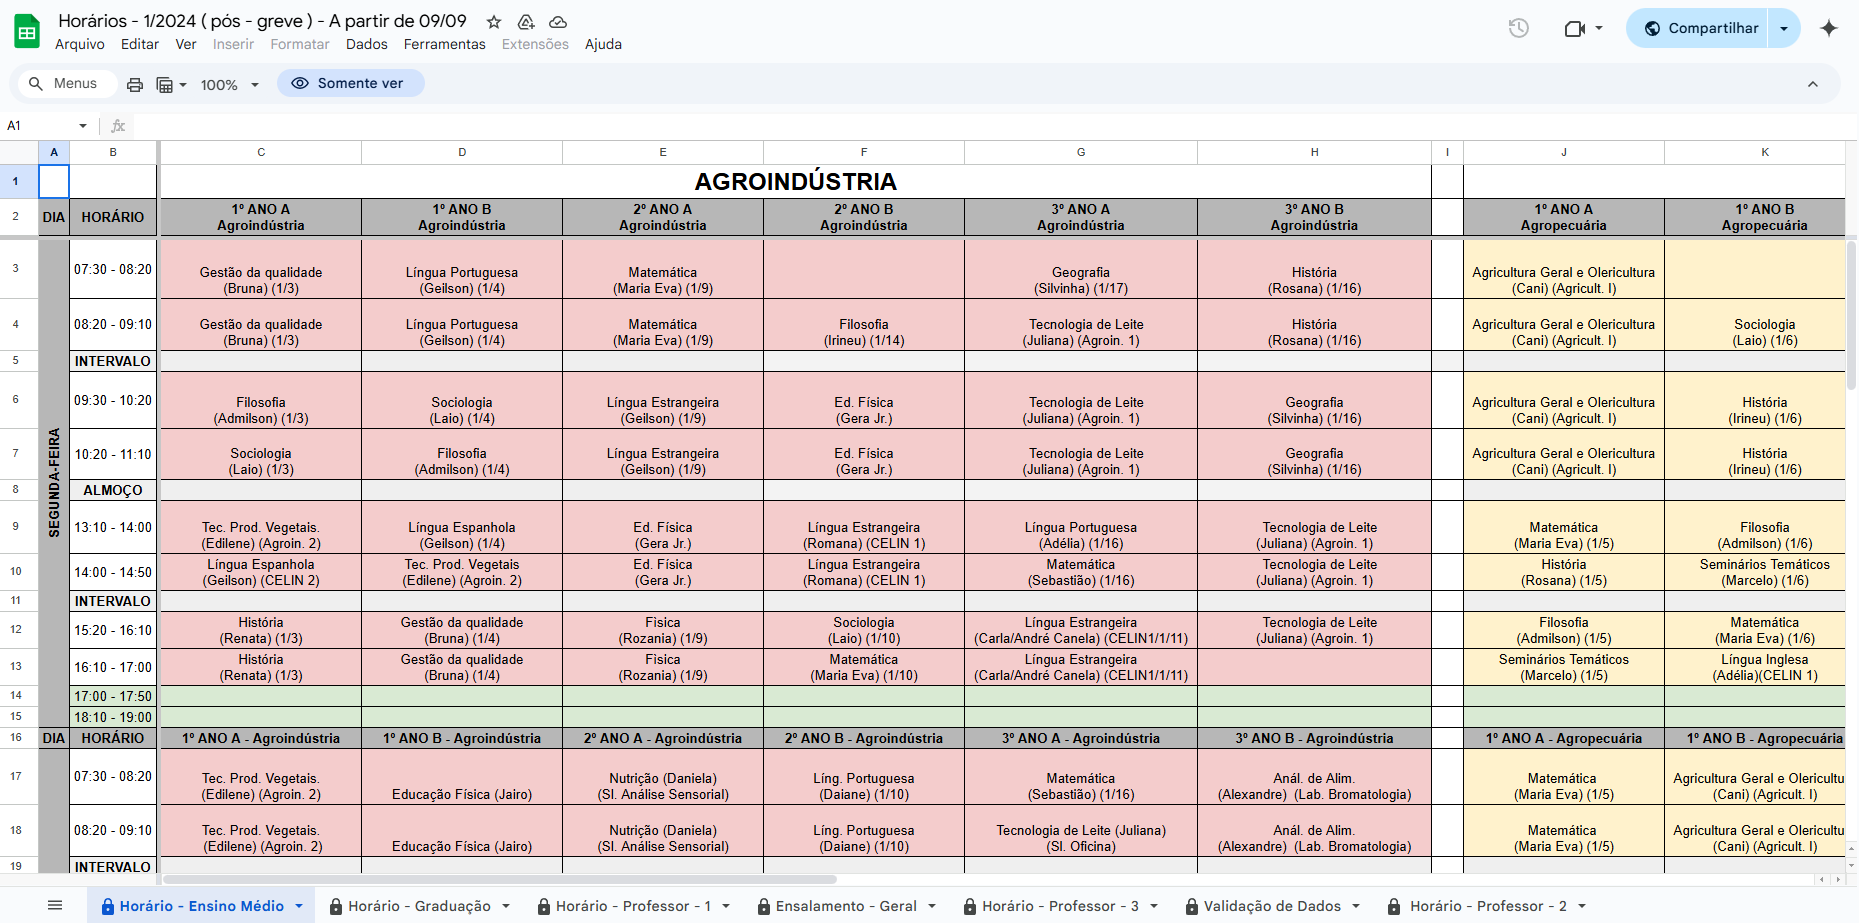
\includegraphics[width=0.9\textwidth]{Figuras/plan-ant-1.png}
                \caption*{Fonte: Elaborado pelo autor (2024)}
                \label{fig_plan-ant_1}
            \end{figure}

            \begin{figure}[H]
                \centering
                \caption{Horário - Graduação}
                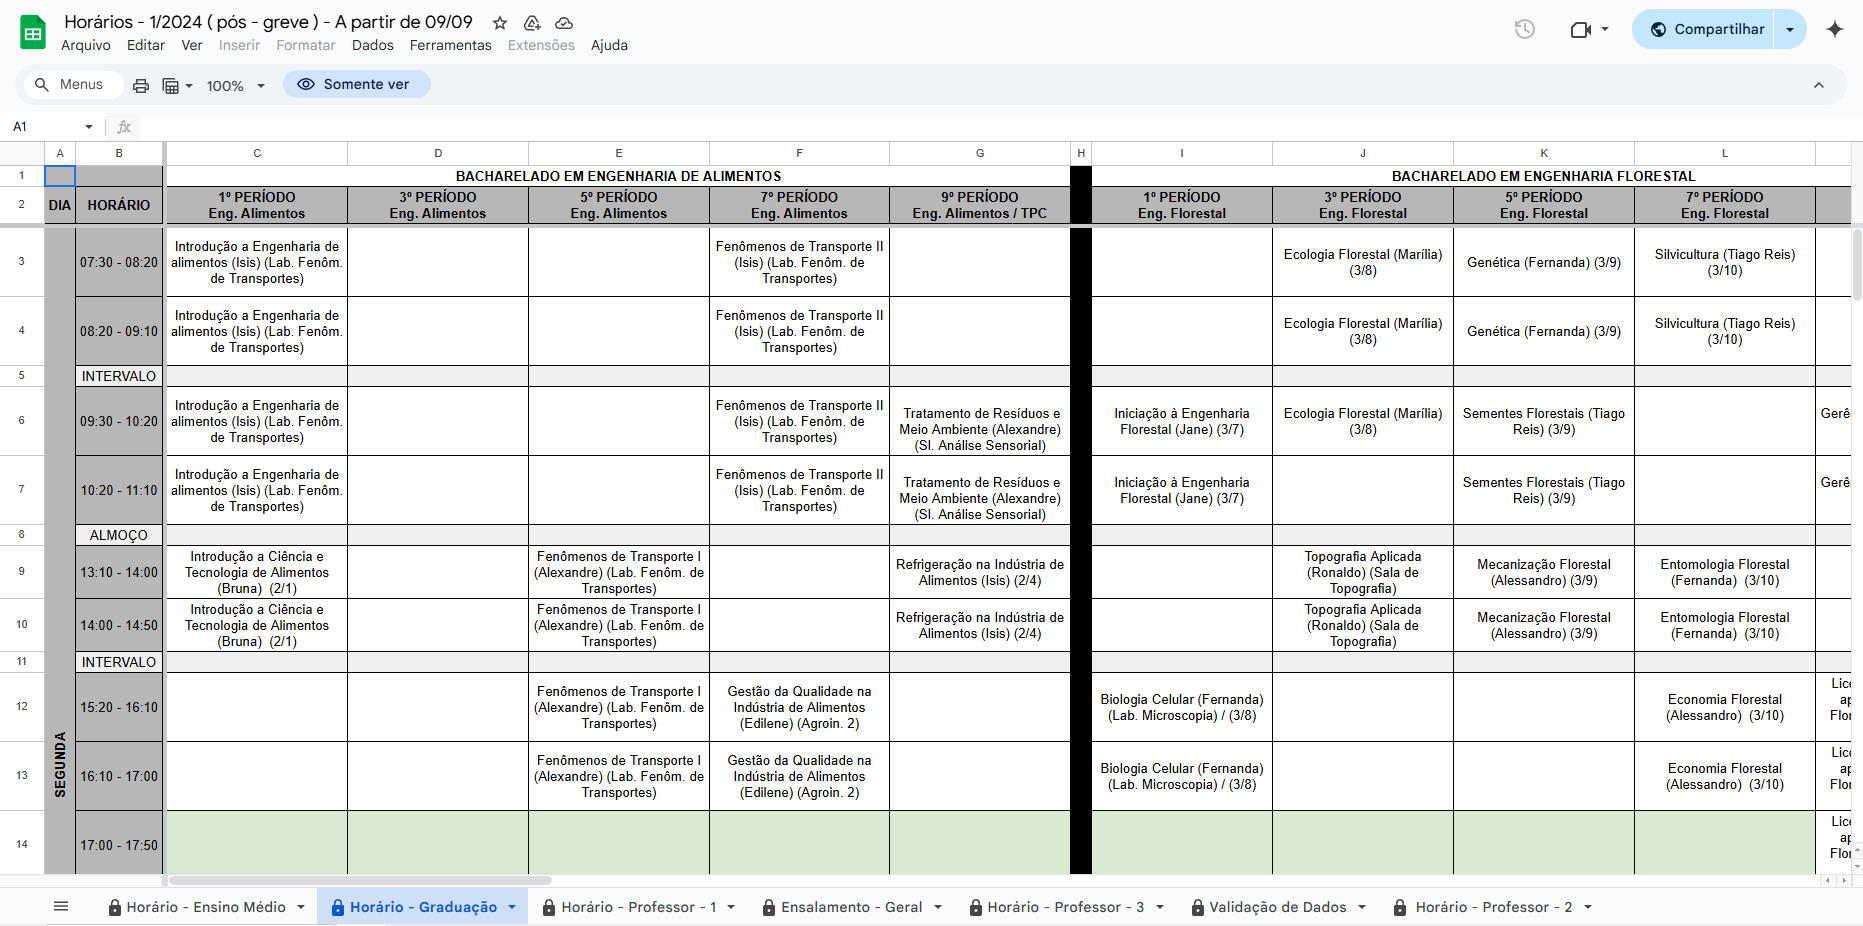
\includegraphics[width=0.9\textwidth]{Figuras/plan-ant-2.png}
                \caption*{Fonte: Elaborado pelo autor (2024)}
                \label{fig_plan-ant_2}
            \end{figure}
            
            \item \textbf{Solução proposta}: Diante das limitações identificadas, a modernização do sistema de exibição de horários é fundamental para garantir maior eficiência e acessibilidade na consulta das informações.
            \item \textbf{Funcionalidades desejadas}: A plataforma deverá ter um menu com quatro opções que permita a consulta de horários dos cursos técnicos, dos cursos superiores, de um professor específico e de uma sala específica. O design deve seguir a identidade visual do IFNMG - Campus Salinas, adotando as cores institucionais para manter a padronização visual. Além disso, é essencial que a plataforma ofereça a opção de download dos horários e seja totalmente responsiva, garantindo uma navegação eficiente em dispositivos móveis, que muitas vezes são o principal meio de acesso utilizado pelos usuários.
        \end{enumerate}
    \end{itemize}
\end{itemize}

\section{Front-end}

\begin{itemize}
    \item \textbf{Protótipo do front-end}: Foi realizada a prototipação da interface, com a validação de um protótipo proposto ao setor com a solução desejada. A grande vantagem de utilizar o protótipo é que o setor teve uma visão prévia da solução final, e pôde rapidamente validar ou solicitar alguma mudança, permitindo modificações antes do desenvolvimento do sistema. Para isso, utilizou-se o \textit{Figma}, uma ferramenta que oferece recursos como armazenamento em nuvem e animações. Esses recursos permitiram um armazenamento seguro, além de possibilitar o compartilhamento, acompanhamento de atualizações em tempo real.
    
    \item \textbf{Desenvolvimento do front-end}: Para o processo de desenvolvimento da interface, foi utilizado o \textit{Next.js}, que permite a construção de aplicações \textit{front-end} reativas que se adaptam dinamicamente a mudanças e eventos, mantendo uma experiência do usuário responsiva, eficiente e de alto desempenho que responde de forma eficiente a eventos em tempo real. Um dos principais fatores da escolha do \textit{Next.js} é sua integração perfeita com o \textit{Tailwind CSS}, que facilita a criação de interfaces modernas, responsivas e altamente customizáveis. Isso simplifica o processo de estilização, pois se puderam utilizar as classes pré-definidas para aplicar estilos consistentes em toda a aplicação.
    
    \textbf{Justificativa de uso da stack do front-end}: Optou-se pelo \textit{Next.js} por simplificar a configuração de rotas e melhorar o desempenho de aplicações \textit{React}, aliado à facilidade de uso em projetos modernos. O \textit{Tailwind CSS} foi integrado devido à compatibilidade com o \textit{Next.js} e à agilidade que oferece na construção de interfaces responsivas. O uso do \textit{TypeScript} proporcionou maior segurança e organização no código por meio de sua tipagem estática, enquanto o \textit{React.js} foi escolhido pela capacidade de criar interfaces dinâmicas e interativas.
\end{itemize}

\section{Back-end}

\begin{itemize}
    \item \textbf{Google Sheets como banco de dados}: Para o processo de desenvolvimento do banco de dados da plataforma, foi utilizado o \textit{Google Sheets}, que oferece uma interface intuitiva para a criação e manipulação de planilhas. A flexibilidade da ferramenta permitiu que funcionasse como um banco de dados leve e eficiente. Com a capacidade de organizar dados em linhas e colunas, o \textit{Google Sheets} facilitou o armazenamento de dados estruturados, como registros de horários, nomes de cursos, turmas, professores e salas. Conforme \citeonline{ufsm2024}, sua estrutura pode ser associada à de um SGBD convencional, com as páginas da planilha representando as tabelas e suas colunas equivalentes às colunas de um SGBD, onde cada linha da planilha representa um registro específico da página.

    Para garantir que o sistema sempre exiba informações atualizadas, o setor de ensino ficou responsável por copiar os dados mais recentes de uma planilha privada e colá-los na planilha utilizada como banco de dados. Esse processo assegura que os usuários tenham acesso aos dados atualizados sem comprometer a segurança e integridade das informações, mantendo a flexibilidade operacional e permitindo que o setor preserve a forma habitual de realizar ajustes nos dados. Não é necessário criar uma nova planilha para o funcionamento da plataforma. No entanto, caso isso ocorra, é crucial que a nova planilha siga exatamente a mesma estrutura da original, respeitando os nomes das guias e os intervalos de células definidos para a extração dos dados. Alterações como renomear guias, excluir ou modificar a posição das células podem comprometer a funcionalidade da plataforma.
    
    \item \textbf{Implementação do back-end:} Para o desenvolvimento do \textit{back-end} da aplicação, foi utilizado o \textit{Spring Boot}, que facilita a criação de sistemas web robustos e escaláveis. A escolha se justificou pela flexibilidade, facilidade de configuração e ampla adoção no mercado. Tornando-se essencial para estabelecer a conexão com a \textit{API} do \textit{Google Sheets}, recebendo os dados e enviando-os ao \textit{front-end} de forma estruturada e confiável. Ademais, para garantir a segurança, foi configurada para permitir apenas operações de leitura, impedindo qualquer tentativa de modificação na planilha do sistema.
    \item \textbf{Arquitetura do back-end}: Seguiu o padrão MVC, que separa a apresentação e a interação dos dados do sistema. Nessa estrutura, o \textit{Model} e o \textit{Controller} pertencem ao \textit{back-end}, enquanto a \textit{View} corresponde à interface, neste caso o \textit{front-end}. Essa divisão garante que as alterações nos dados ocorram de modo independente de sua apresentação, permitindo diferentes formas de exibir os dados.
    \item \textbf{Justificativa de uso da stack do back-end}: Optou-se pela linguagem \textit{Java} com o \textit{Spring Framework} por fornecer uma base estável para criar aplicações seguras e escaláveis. O \textit{Spring Boot} foi adotado para agilizar a configuração e o desenvolvimento, evitando ajustes manuais desnecessários. O \textit{Google Sheets} foi utilizado como banco de dados devido à integração simples e ao suporte adequado às necessidades do projeto, com acesso realizado por meio da \textit{Google Sheets API}, garantindo a leitura estruturada e segura dos dados. Para assegurar portabilidade e isolamento do ambiente, aplicou-se a conteinerização com \textit{Docker}, facilitando o deploy em diferentes ambientes.
\end{itemize}

\section{Integração Front-end com Back-end}

A integração foi realizada por meio de uma \textit{API RESTful} desenvolvida com \textit{Spring Boot}, que atuou como intermediária entre a interface construída em \textit{Next.js} e os dados armazenados no \textit{Google Sheets}. O \textit{front-end} envia requisições HTTP ao \textit{back-end} para acessar informações como horários de cursos, turmas, professores e salas. Essas solicitações são processadas pelo \textit{back-end}, que recuperava os dados por meio da \textit{Google Sheets API} e os retornava no formato \textit{JSON}. Dessa forma, as informações são exibidas na interface de maneira clara, organizada e dinâmica.

Alterações feitas diretamente no \textit{Google Sheets} aparecem automaticamente na plataforma, pois a \textit{API} acessou os dados atualizados da planilha. Assim, eliminou-se a necessidade de atualizações manuais ou processos de sincronização, otimizando a experiência do usuário final. O \textit{back-end} foi implementado com mecanismos de controle de acesso, garantindo a segurança e preservando a integridade das informações. A integração promovida conectou as diferentes partes do sistema de maneira eficiente, promovendo uma experiência confiável e responsiva.

\section{Deploy}

Para disponibilizar o sistema na internet, o \textit{front-end} foi implementado em uma conta particular na \textit{Vercel}\footnote{https://vercel.com/docs}, uma plataforma especializada no deploy de aplicações web baseadas em \textit{JavaScript}, como o \textit{Next.js}, que oferece uma integração direta e otimizada para esse tipo de aplicação. O \textit{back-end}, por sua vez, foi hospedado em uma conta privada na \textit{Koyeb}\footnote{https://www.koyeb.com/docs}, uma plataforma serverless amigável para desenvolvedores, projetada para permitir que empresas implantem aplicativos confiáveis e escaláveis globalmente.

\section{Armazenamento do Código e Integração}

Para a hospedagem do código, foi utilizado o \textit{GitHub}\footnote{https://github.com/}, um repositório de hospedagem de serviços \textit{Git}. Podendo ser considerado como uma rede social para desenvolvedores, além de uma plataforma colaborativa. Ao utilizá-lo, os programadores podem interagir e colaborar em repositórios de código aberto, permitindo que realizem downloads, cooperem, compartilhem, além de outras funcionalidades \cite{silva2024biblioteca}.

Uma conta do \textit{GitHub} foi vinculada às plataformas \textit{Vercel} e \textit{Koyeb} para permitir o acesso direto aos arquivos do projeto, viabilizando a integração necessária para o deploy. Na \textit{Koyeb}, o \textit{Docker} foi utilizado para criar e gerenciar contêineres, garantindo o isolamento e a portabilidade do \textit{back-end}, desenvolvido com \textit{Spring Boot}. Dessa forma, proporcionou o funcionamento adequado de ambas as partes do sistema.

\section{Ambiente de desenvolvimento}

Para a codificação do sistema, foi utilizado o \textit{Visual Studio Code}\footnote{https://code.visualstudio.com}, um editor de código-fonte criado pela Microsoft com o objetivo de auxiliar programadores na criação de softwares. Sendo amplamente adotado para escrever, editar e gerenciar os códigos durante o desenvolvimento de um projeto \cite{silva2024biblioteca}.

A escolha desse editor se justificou por sua facilidade na construção de códigos e por sua interface limpa, personalizável e organizada.

\section{Avaliação da Plataforma}

Para avaliar a eficácia da plataforma, foi realizada uma análise baseada na percepção do responsável pela gestão acadêmica que participou do levantamento de requisitos. A reunião foi agendada com o Coordenador de Ensino Superior/Diretor de Ensino Substituto do Campus Salinas, o professor Frederico Ventura Batista, para fornecer feedbacks detalhados sobre o sistema desenvolvido.

A condução da entrevista para a avaliação da plataforma foi realizada conforme os seguintes passos:
\begin{itemize}
    \item \textbf{Preparação}:
    \begin{itemize}
        \item \textbf{Agendamento}: A reunião foi marcada com antecedência, com a confirmação da disponibilidade do Sr. Frederico Ventura Batista.
        \item \textbf{Objetivos}: Foram claramente definidos para verificar se a plataforma atende às necessidades do setor e identificar possíveis pontos de melhoria.
    \end{itemize}
    \item \textbf{Entrevista}: A entrevista foi iniciada com uma explicação ao entrevistado sobre o objetivo do questionário e o propósito da avaliação. Em seguida, o entrevistado respondeu às perguntas apresentadas.
    \item \textbf{Perguntas}: A entrevista foi guiada por um questionário com seis perguntas abertas, adaptado com base no instrumento utilizado no Trabalho de Conclusão de Curso ``SIGALAB: Sistema de Informação Gerencial Acadêmico para Reservas de Laboratórios'' \cite{costa2018sigalab}. As questões e respostas estão registradas no Apêndice \ref{apendiceB}. Isso permitiu coletar informações sobre a experiência de uso e as percepções do setor em relação à solução desenvolvida.
    \item \textbf{Documentação}:
    \begin{itemize}
        \item \textbf{Registro Detalhado}: Durante a entrevista, foram registrados os principais pontos discutidos, entre eles:
        \begin{enumerate}
            \item \textbf{Usabilidade e navegação}: A plataforma é mais fácil de usar em comparação com a planilha anteriormente utilizada.
            \item \textbf{Eficiência na exibição dos horários}: As informações são apresentadas de forma clara e organizada, facilitando a consulta.
            \item \textbf{Redução de dificuldades operacionais}: O sistema ajudou a minimizar as dificuldades no gerenciamento dos horários acadêmicos e melhorou o fluxo de trabalho.
            \item \textbf{Satisfação geral}: A plataforma atendeu às expectativas do setor e se mostrou uma solução eficaz para a gestão dos horários acadêmicos.
            \item \textbf{Melhorias e atualizações}: A integração de outras ferramentas de apoio à gestão do ensino, como a criação de uma nova funcionalidade para validação dos dados da planilha e adição de links diretos para os sistemas complementares, como o de reserva de horários, o que exibe os locais do instituto e o de gerenciamento de reserva de salas.
            \item \textbf{Garantia de Disponibilidade}: O software será transferido para a instituição, com a elaboração de uma documentação para orientar a manutenção do sistema.
        \end{enumerate}
    \end{itemize}
\end{itemize}

Dessa forma, a avaliação foi conduzida de maneira ética e transparente, garantindo que os resultados obtidos refletissem de forma precisa a usabilidade e a efetividade da plataforma como substituta da planilha na exibição dos horários acadêmicos.

\section{Implementação de Melhorias e Atualizações}

Com base nas sugestões e críticas obtidas na avaliação da plataforma, foram realizadas melhorias voltadas a aprimorar a usabilidade e expandir as funcionalidades do sistema. O histórico das versões desenvolvidas até o momento:

\begin{itemize}
    \item \textbf{v.1.0.0}: A primeira versão correspondeu à versão inicial do projeto, que disponibilizou quatro opções no menu principal para a consulta dos horários acadêmicos. Essas opções permitiam visualizar os horários dos cursos técnicos, dos cursos superiores, de um professor específico e de uma sala específica.
    \item \textbf{v.2.0.0}: Na segunda versão, foram implementadas melhorias e atualizações a partir da avaliação realizada. As principais mudanças foram:
    \begin{itemize}
        \item Desenvolvimento de uma nova tela de login para entrar na tela de validação de dados.
        \item Criação de uma nova planilha no \textit{Google Sheets} com as credenciais de login para acessar a tela de validação de dados.
        \item Implementação de uma nova tela para a validação dos dados da planilha dos horários.
        \item Adição de um botão no menu principal da plataforma para direcionar para validação de dados.
        \item Inclusão de três novos botões no menu principal da plataforma com links externos para os sistemas complementares, como o de reserva de horários, o de visualização dos locais do instituto e o de gerenciamento de reserva de salas.
    \end{itemize}
\end{itemize}

Essas melhorias foram aplicadas considerando a viabilidade técnica e a relevância para os usuários, garantindo que a plataforma continue evoluindo para atender melhor às demandas do setor de ensino.

\section{Documentação}

Para garantir a correta manutenção e funcionamento da plataforma, foi elaborada uma documentação técnica da planilha com diretrizes essenciais sobre elementos estruturais que não podem ser alterados e regras que devem ser seguidas. Essa documentação abordou os seguintes aspectos:

\begin{itemize}
    \item \textbf{Estrutura e organização dos dados}: Estão descritos os procedimentos que devem ser realizados no início de cada semestre, como a atualização do \textit{ID} da planilha com os horários acadêmicos na sua variável de ambiente, o uso de cópias da planilha original privada do setor de ensino para evitar alterações indesejadas, e os cuidados com a plataforma de deploy do \textit{back-end}.
    \item \textbf{Regras para adição e atualização de informações}: Inclui exemplos de preenchimento dos campos na planilha, com orientações sobre a escrita padronizada. Os nomes das disciplinas não devem conter parênteses, os nomes dos professores precisam estar entre parênteses, e os nomes das salas igualmente devem estar entre parênteses, sem espaços extras. Algumas exceções são aceitas, como entradas com múltiplos professores ou informações adicionais. Na guia de \textit{Validação de Dados}, deve-se evitar nomes com espaços ou parênteses antes e depois.
    \item \textbf{Padrões para nomes de guias e intervalos de células}: Traz a explicação da estrutura do \textit{Google Sheets}, onde as colunas são representadas por letras e as linhas por números. Cada célula é identificada pela combinação da letra da coluna com o número da linha. Em seguida, foram definidos os nomes e intervalos das três guias essenciais para o correto funcionamento da plataforma, sendo elas:
    \begin{itemize}
        \item \textit{Horário - Ensino Médio}, com intervalo de células B2:V76;
        \item \textit{Horário - Graduação}, com intervalo de células B2:AW106;
        \item \textit{Validação de Dados}, com intervalo de células A2:A.
    \end{itemize}
    É importante ressaltar que não devem ser feitas alterações nesses nomes ou na posição das células. Mudanças estruturais só devem ocorrer se forem realmente necessárias e com a devida atualização no código.
\end{itemize}

Com isso, a documentação servirá como referência para futuros administradores da plataforma, assegurando a continuidade do sistema e facilitando sua manutenção.